\section{Smart Home}
\label{sec:smartHome}
    \acl{SH}, übersetzt in Deutsch \textit{“intelligentes Zuhause“}, ist einer von mehreren bekannten Zweigen des \acs{IoT}. 
    Speziell diese Rubrik widmet sich explizit 
    sämtlichen Haushaltsgeräten und -einrichtungen. Aus diesem Grund können viele Geräte ebenso intelligente Gegenstände 
    der Rubrik \acl{SH} sein. Ein kleiner Ausschnitt solcher Nutzgegenstände sind unter anderem Lampe, Kontaktsensoren, 
    Thermostate, Service-Roboter, Staubsauger-Roboter, Kühlschränke Geräte rundum die Haussicherheit. 
    \\ 
    Unter dem Oberbegriff \acl{SH} ist auch eine Weise zu verstehen, mit der die Erhöhung der Wohn- und Lebensqualität, 
    effizienteren Energienutzung unter Verwendung vernetzter und fernsteuerbarer Geräten, Sicherheit sowie automatisierbaren 
    Abläufe gesteigert werden kann. 
    \\ 
    Der Begriff intelligenten Zuhause wird auch schon verwendet, wenn die Haustechnik und Haushaltsgeräte unter einander  
    vernetzt sind. Die Definition im Deutschen Gebrauch, welche nach (Strese et al. 2010) in der Untersuchung im Rahmen 
    der wissenschaftlichen Begleitung zum Programm Next Generation Media (NGM) des Bundesministeriums für Wirtschaft und 
    Technologie aufgegriffen wird, lautet wie folgt: 
    \begin{quote}
        „Das Smart Home ist ein privat genutztes Heim (z.B. Eigenheim, Mietwohnung), in dem die zahlreichen Geräte der 
        Hausautomation (wie Heizung, Beleuchtung, Belüftung), Haushaltstechnik (wie z.B. Kühlschrank, Waschmaschine), 
        Konsumelektronik und Kommunikationseinrichtungen zu intelligenten Gegenständen werden, die sich an den 
        Bedürfnissen der Bewohner orientieren. Durch Vernetzung dieser Gegenstände untereinander können neue 
        Assistenzfunktionen und Dienste zum Nutzen des Bewohners bereitgestellt werden und einen Mehrwert 
        generieren, der über den einzelnen Nutzen der im Haus vorhandenen Anwendungen hinausgeht.“ \cite{strese.2010m}
    \end{quote}
    Eine vergleichbare Definition wurde zu späterem Zeitpunkt durch eine Literaturrecherche publiziert. Diese beschreibt 
    die zugrundeliegende Thematik weniger aus Anwendersicht sonder widmet sich vielmehr dem System und der Konnektivität. 
    \begin{quote}
        „A smart home is a place with heterogeneous systems to many
        front devices with the support of embedded information and
        communication architectures[...]“ \cite{Balakrishnan2018}
    \end{quote}
    Den beiden Definitionen ist zu entnehmen, dass die Kernaussage eine ähnliche ist, es jedoch in Büchern, Fachartikeln, 
    Publikationen an Universitäten und in den verbreiteten Medien bis heute keine durchgängige Definition gibt. Aus der
    % empirischen 
    einschlägigen Literatur wird ersichtlich, dass viele Synonyme für die Benennung der Thematik verwendet werden, darunter 
    beispielsweise: \cite{strese.2010m}
    \begin{itemize}
        \item Connected Home
        \item Elektronisches Haus
        \item Intelligentes Haus (engl. Smart House)
        \item Smart Living
        \item Home of the Future 
    \end{itemize}
    Eine elementare Information im Zusammenhang zu dieser Arbeit ist, dass die Verwendung des Begriffs \textit{intelligentes Büro} 
    ebenso in den Kontext des \acl{SH} gehört. Hierbei wird lediglich die Räumlichkeit im unternehmerischen Jargon verwendet, 
    die ebenso Grundlage für die Verwendung von Komponenten des \acl{SH} bietet. 
    \\
    An dieser Stelle wird ebenso deutlich, dass die Verwendung des Begriffs als auch die zugrundeliegenden technisches Verfahren 
    weiträumig einsetzbar sind und deshalb die Begriffsdefinition nicht eindeutig festgehalten werden kann. 
    
    \subsubsection*{Teilsysteme des \acl{SH}}
        Der Zentrale Punkt des \acl{SH} ist die Automatisierung häuslicher Prozesse. Dadurch sollen dem Nutzer 
        in vielerlei Hinsicht Aufwände erspart und Informationen zentralisiert angezeigt werden. Die Hausautomatisierung 
        umfasst eine Menge von Teilsystemen. Eine Teilmenge davon ist der folgenden tabellarischen Auflistung zu entnehmen: 
        \begin{table}[hbt!]
            \begin{center}
                \begin{tabular}{| p{3cm} | p{12.75cm} | }
                    \hline
                        \textbf{Segment} & \textbf{Beschreibung} \\
                    \hline
                        Licht & Beleuchtung, Lichtmanagement/Szenarien, Storen/Rollos \\ 
                    \hline
                        Zutritt & Zutrittskontrolle, Klingelanlage, Schlösser, Anwesenheits- und Bewegungserfassung \\ 
                    \hline
                        Überwachung & Technische Alarme: Feuer, Rauch, Gas; Intrusion: Glasbruchmelder, Video; Babyphon, Urlaubswachschutz \\ 
                    \hline
                        Notfall & Sprinkleranlage, unabhängige Stromversorgung, Fluchtwegsystem \\ 
                    \hline
                        Metering & Verbrauchszähler für Strom, Gas, Wasser, Wärme, uvm. \\ 
                    \hline 
                        Konsumelektronik & TV, Internet, Smartphones, Tablets, Spielekonsolen etc. \\
                    \hline
                        Hausgeräte & Kühlschrank, Waschmaschine, Staubsauger, Service-Roboter; Hausgeräte-monitoring, -diagnostik, und -fernbedienung \\
                    \hline
                        Heimlogistik & Einkaufs- und Speiseplanung, häusliche Dienste \\ 
                    \hline
                        Hobby & Haustierversorgung, Aquarienmanagement, etc. \\
                    \hline
                        Mobilität & PKW mit Diagnostik, Navigationssystem mit local based services, Info-/Entertainmentangebote etc. \\ 
                    \hline
                \end{tabular}
                \label{table:teilsysteme}
            \end{center}
            \caption{Teilsysteme des Smart Home \cite{strese.2010m}}
        \end{table}
        \\
        Ein weiterer wichtiger Anhaltspunkt zum Verständnis der Definition von Smart Home ist die Ausstattung der Komponenten mit Intelligenz und die 
        Vernetzung der Teilsysteme. Dadurch steht als Ziel im Vordergrund nicht die übergeordnete zentrale Steuerung, sondern vielmehr die verteilte 
        Intelligenz, um Aufgaben möglichst autonom (eigenständig) abzuarbeiten. Die dabei erzeugten als auch erforderlichen Daten mit anderen 
        Komponenten des Gesamtsystems auszutauschen, ist ebenso ein vorangestelltes Ziel, welches eine intelligente Umgebung schafft. 
        \\
        Eine mögliche Vernetzung und auch Verwendung solcher Komponenten wird in folgender Abbildung (\ref{pic:szenarien-smarhome}) 
        skizziert. Diese Grafik dient als grobe Übersicht potentieller Anwendungsszenarien, ist allerdings nicht als vollständig zu interpretieren. 
        \begin{figure}[hbt!]
            \centering
            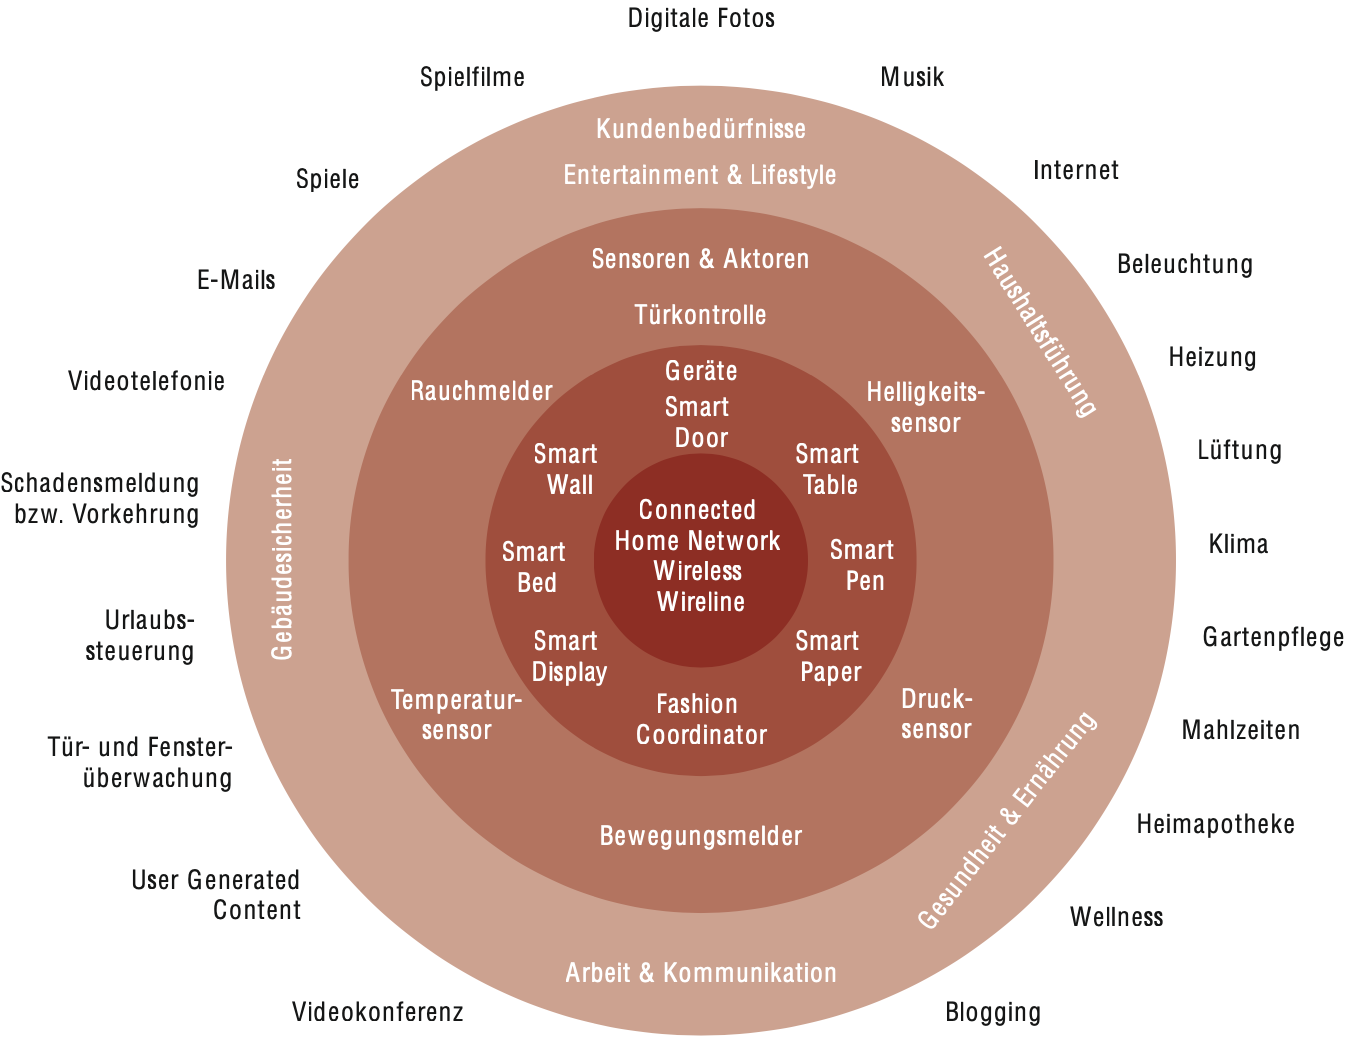
\includegraphics[width=15cm,height=15cm,keepaspectratio]{images/Anwendungsszenarien_SH.png}
            \caption{Mögliche Anwendungsszenarien im Smart Home \cite{strese.2010m}}
            \label{pic:szenarien-smarhome}
        \end{figure}
        \\
        Es gibt weitaus mehr, beziehungsweise werden diese in einem Überbegriff untergeordnet. Ein essentielles Anwendungsszenario ist die Kopplung 
        von Robotern jeglicher Art, darunter Staubsaugerroboter oder auch Service-Roboter, die immer mehr in die Thematik des \acl{SH} integriert werden. 
        
    \subsubsection*{Einordnung von Smart Home in das Internet der Dinge}
        Im Konsumentenmarkt privat genutzter Geräte wird die Technologie des \acs{IoT} in Produkten eingesetzt, die das Konzept des \acl{SH} verfolgen. 
        Diese beinhalten Haushaltsgeräte und -ausstattung, wie beispielsweise Thermostate, Sensoren, Sicherheitssysteme und Lampen, die in den meisten 
        Fällen mehrere Systeme und Übertragungstechnologien unterstützen. Weitere Beispiele sind der Tabelle (\ref{table:teilsysteme}) zu entnehmen. 
        \begin{figure}[hbt!]
            \centering
            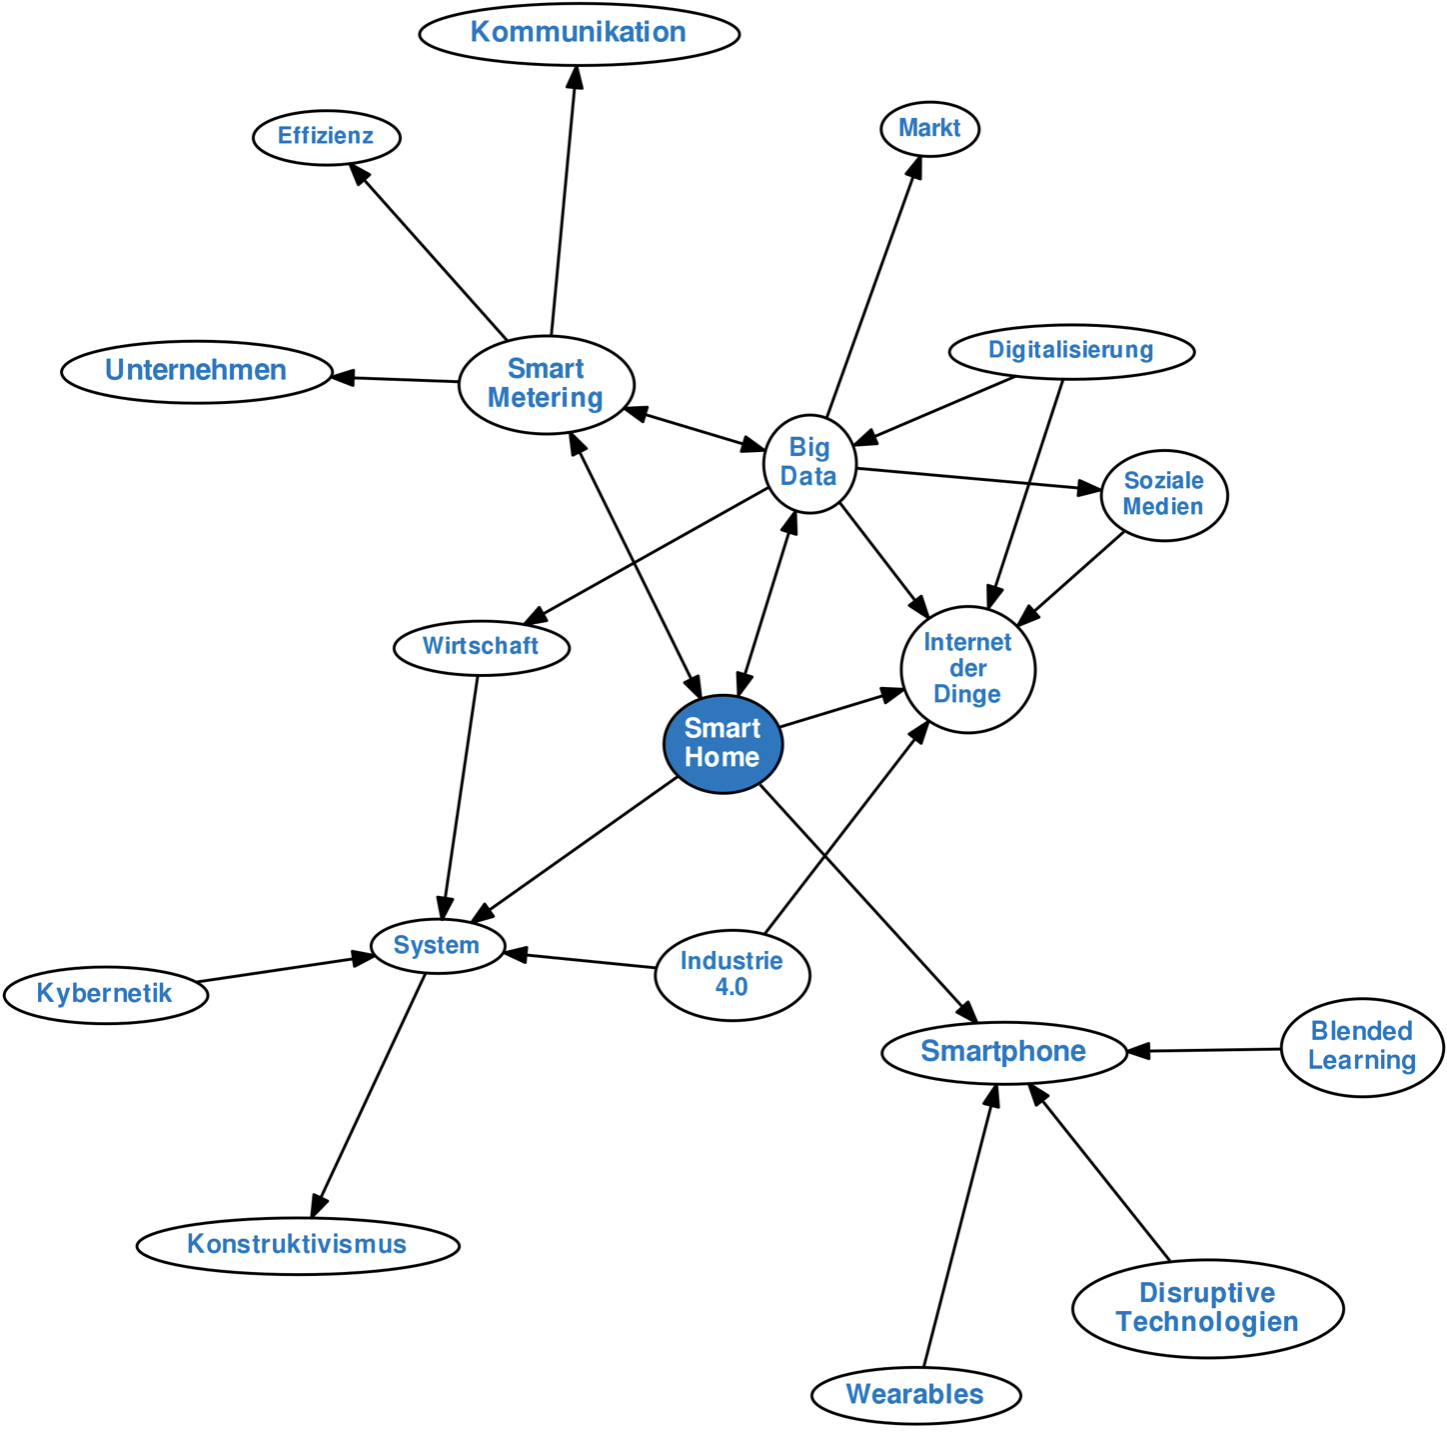
\includegraphics[width=13cm,height=13cm,keepaspectratio]{images/smartHome_mindmap.png}
            \caption{Smart Home in Abhängigkeit zu IoT}
            \label{pic:mindmap_SH-IoT}
        \end{figure}
        \\
        \linebreak
        Die Abbildung \ref{pic:mindmap_SH-IoT} zeigt die Verknüpfungen 
        %Funktionweise von Smart HOme
        %Fügung in ein IoT Grundprinzip - https://www.aimprosoft.com/blog/iot-smart-home/  


    \subsubsection{Eigendefinition Smart Home}
    
    \subsection{Historische Entwicklung}

    \subsection{Ziele von Smart Home}